\documentclass[11pt]{article}
\usepackage[margin=1in]{geometry}
\usepackage[T1]{fontenc}
\usepackage{lmodern,microtype,booktabs,graphicx,amsmath,caption,hyperref}
\usepackage[numbers,sort&compress]{natbib}
\captionsetup{font=small,labelfont=bf}
% generated by paper/make_tables.py; do not edit
\newcommand{\DnaProm}{92.4}
\newcommand{\DnaPromSd}{1.0}
\newcommand{\DnaPromF}{92.4}
\newcommand{\DnaPromEce}{0.061}
\newcommand{\CnnProm}{83.5}
\newcommand{\CnnPromSd}{0.6}
\newcommand{\CnnPromF}{83.4}
\newcommand{\CnnPromEce}{0.157}
\newcommand{\DnaEnh}{74.4}
\newcommand{\DnaEnhSd}{0.8}
\newcommand{\DnaEnhF}{74.3}
\newcommand{\DnaEnhEce}{0.136}
\newcommand{\CnnEnh}{66.9}
\newcommand{\CnnEnhSd}{1.4}
\newcommand{\CnnEnhF}{65.5}
\newcommand{\CnnEnhEce}{0.303}
\newcommand{\MajProm}{54.4}
\newcommand{\MajEnh}{50.0}
\newcommand{\StratLowDna}{80.4}
\newcommand{\StratLowCnn}{59.5}
\newcommand{\StratHighDna}{98.9}
\newcommand{\StratHighCnn}{95.2}
\newcommand{\ManOneH}{62.3}
\newcommand{\ManThreeH}{63.8}
\newcommand{\ManOneK}{68.3}
\newcommand{\ManThreeK}{73.0}
\newcommand{\AiRandThree}{69.5}
\newcommand{\EceRandThree}{0.231}
\newcommand{\AiLcThree}{70.0}
\newcommand{\EceLcThree}{0.248}
\newcommand{\AiEnsThree}{72.3}
\newcommand{\EceEnsThree}{0.210}
\newcommand{\EceManThree}{0.095}
\newcommand{\EceManOne}{0.176}
\newcommand{\EceAiOnlyOne}{0.265}
\newcommand{\nFullBeats}{1}
\newcommand{\nLowBeats}{1}
\newcommand{\nFullWorse}{3}
\newcommand{\nLowWorse}{3}
\newcommand{\nFullNoClear}{20}
\newcommand{\nLowNoClear}{20}
\newcommand{\nComp}{24}
\newcommand{\EnsVsRandMean}{2.8}
\newcommand{\EnsVsRandLo}{1.3}
\newcommand{\EnsVsRandHi}{4.5}
\newcommand{\LcVsRandMean}{0.6}
\newcommand{\LcVsRandLo}{-0.4}
\newcommand{\LcVsRandHi}{1.5}
\newcommand{\RandVsManMean}{-3.5}
\newcommand{\RandVsManLo}{-5.5}
\newcommand{\RandVsManHi}{-1.6}
\newcommand{\LcVsManMean}{-2.9}
\newcommand{\LcVsManLo}{-5.4}
\newcommand{\LcVsManHi}{-0.7}
\newcommand{\EnsVsManMean}{-0.7}
\newcommand{\EnsVsManLo}{-1.5}
\newcommand{\EnsVsManHi}{0.1}
\newcommand{\OnlyVsManMean}{3.1}
\newcommand{\OnlyVsManLo}{-0.8}
\newcommand{\OnlyVsManHi}{7.4}
\newcommand{\nRecords}{317}
\newcommand{\RunHours}{3.7}
\newcommand{\EnsSeedMin}{1.4}
\newcommand{\EnsSeedMax}{4.9}
\newcommand{\EnsSeedPos}{5}
\newcommand{\LcSeedMin}{-1.0}
\newcommand{\LcSeedMax}{1.7}
\newcommand{\LcSeedPos}{4}
\newcommand{\ProposerAccOneH}{63.6}
\newcommand{\PseudoAccOneH}{64.3}
\newcommand{\ProposerAccThreeH}{68.1}
\newcommand{\PseudoAccThreeH}{68.5}
\newcommand{\ProposerAccOneK}{70.5}
\newcommand{\PseudoAccOneK}{70.6}
\newcommand{\RevPropRand}{70.5}
\newcommand{\RevLabRand}{95.0}
\newcommand{\RevPropLc}{51.9}
\newcommand{\RevLabLc}{95.4}
\newcommand{\RevPropEns}{50.2}
\newcommand{\RevLabEns}{95.2}
\newcommand{\SensEnsMin}{0.5}
\newcommand{\SensEnsMax}{3.1}
\newcommand{\SensLcMin}{-0.3}
\newcommand{\SensLcMax}{1.3}
\newcommand{\SensEnsAllPos}{all six}
\newcommand{\nLowOverlap}{5,805}
\newcommand{\pctLowOverlap}{83.5}

\newcommand{\pp}{\,pp}
\title{Does Routing Human Review by Model Uncertainty Help?\\ A Simulated Study of AI-Assisted Labelling for DNA Sequence Classification}
\author{Pratik Satpathy\\ \small Roll no.\ RSI2025512, course \emph{AI Tools for Research}, IIIT Allahabad}
\date{November 2026}
\begin{document}
\maketitle

\begin{abstract}
Labelling genomic sequences by hand is slow, and AI-assisted labelling, in which a model proposes labels and a person reviews some of them, is an obvious way to save effort. Whether it actually helps at \emph{equal human effort} is rarely measured. We simulate it. A DNABERT-2 model is fine-tuned on a small seed set, proposes labels for a pool of 500-base enhancer sequences, and a simulated annotator reviews a budget of items chosen by one of four routing policies (random, least-confidence, margin, five-model ensemble disagreement). We compare against purely manual labelling with the same number of human labels, against AI-only labelling, and across annotator error and reliance on the AI. Before this, we audit the benchmark itself and find that on the non-TATA promoter dataset 45.6\% of the test set is almost duplicated in training, almost all of it negatives, so we exclude it. On the enhancer dataset, over five seeds and a protocol frozen before the main run, the only routing policy that clearly beats random review is ensemble disagreement at the largest budget (\EnsVsRandMean\pp, 95\% interval \EnsVsRandLo{} to \EnsVsRandHi\pp). No AI-assisted arm beats manual labelling at equal human labels; at 3,000 labels three of four policies are clearly worse. AI-assisted models are also worse calibrated. These results come from simulated annotators on one dataset and should be read as a simulation study, not evidence about real annotators.
\end{abstract}

\section{Introduction}
Supervised models for regulatory DNA need labelled sequences, and labels are costly. A common proposal is to let a model pre-label the data and ask people to review only part of it. Two design questions follow. Which items should be sent to the reviewer? And, at the same number of human labels, is the AI-assisted pipeline actually better than simply spending those labels on randomly chosen items? Active learning has studied item selection for decades \citep{settles2009,seung1992qbc}, but the combination that matters in practice (pseudo-labels for everything that is \emph{not} reviewed, a reviewer who may trust the model too much \citep{parasuraman2010}, and calibration of the resulting model \citep{guo2017calibration}) is rarely examined together on genomic data.

We ask three questions, fixed before the main experiment (protocol commit \texttt{92e1e49}):
\textbf{RQ1} at equal human labels, does routing review by uncertainty beat random review?
\textbf{RQ2} at equal human labels, does AI-assisted labelling beat manual labelling, and how does this depend on annotator error and reliance?
\textbf{RQ3} how well calibrated are the resulting models?
A claim of improvement required a mean paired gain of at least one percentage point and a 95\% interval above zero.

\section{Data and a leakage audit}
We use two datasets from Genomic Benchmarks \citep{gresova2023} with their official train/test splits: human non-TATA promoters (251 bases; 27{,}097 train, 9{,}034 test) and human enhancers from Cohn et al.\ (500 bases; 20{,}843 train, 6{,}948 test; balanced). As model we use DNABERT-2-117M \citep{zhou2024dnabert2}; the package CNN from Genomic Benchmarks serves as a comparator.

\paragraph{Exact duplicates.} Both datasets have no duplicate sequences within train or test, no train/test overlap and no sequence under two labels.

\paragraph{Shared sub-sequences.} Exact checks are not enough for genomic windows, which can overlap. For every test sequence we measured the fraction of its 16-mers (both strands) that also occur in the training set. Table~\ref{tab:leak} shows that the promoter split is heavily affected: 45.6\% of test sequences share more than 80\% of their 16-mers with training. Their labels are almost all negative (Table~\ref{tab:strat}), and the training negatives are themselves nearly redundant (98.2\% of their 16-mers occur in other training sequences, against 9.9\% for positives). Only 6\% of the overlapping test negatives are explained by one training sequence at one shift, so the redundancy is not simple duplication. Our reading, which we did not check against the benchmark's construction, is that negatives are densely overlapping windows of shared regions. Sequence complexity is not the cause: distinct 16-mers per sequence are about 99.6--99.8\% in both classes.

\begin{table}[t]
\centering\small
\begin{tabular}{lrrrcc}
\toprule
 & Test & $>$80\% & $>$95\% & Train neg.\ & Train pos.\\
\midrule
Promoters & 9{,}034 & 4{,}120 (45.6\%) & 3{,}866 (42.8\%) & 98.2\% & 9.9\%\\
Enhancers & 6{,}948 & 60 (0.86\%) & 5 (0.07\%) & 15.2\% & 7.8\%\\
\bottomrule
\end{tabular}
\caption{Share of test 16-mers also found in training (both strands), and redundancy inside the training set by class. Last two columns: mean share of 16-mers found in other training sequences. Source: leakage scripts run by the student.}\label{tab:leak}
\end{table}

\begin{table}[t]
\centering\small
\begin{tabular}{lrrcc}
\toprule
Shared 16-mers with train & Test seqs & Positive (\%) & DNABERT-2 acc (\%) & CNN acc (\%) \\
\midrule
$\leq$5\% & 2,694 & 99.5 & 80.4 & 59.5 \\
5--50\% & 1,995 & 99.2 & 96.1 & 91.6 \\
50--80\% & 225 & 65.3 & 89.5 & 83.4 \\
$>$80\% & 4,120 & 2.6 & 98.9 & 95.2 \\
\bottomrule
\end{tabular}

\caption{Promoters: test accuracy by overlap with training, mean over seeds 0--3 (seed 4 was not yet finished when this analysis was run). The positive share per group was measured directly. The low-overlap group is almost entirely positive, so accuracy there is essentially recall on positives.}\label{tab:strat}
\end{table}

This matters for any result reported on the promoter split. Accuracy is \StratHighDna\% (DNABERT-2) and \StratHighCnn\% (CNN) on the heavily overlapping group, but only \StratLowDna\% and \StratLowCnn\% on the group that shares at most 5\% of its 16-mers with training. Because overlap is almost a class marker there, a model can score well by recognising what it has seen. Only about 30 test negatives share at most half of their 16-mers with training, so the split cannot measure how a model handles unseen negatives. The enhancer split is much cleaner (Table~\ref{tab:leak}), and accuracy there is almost flat across overlap groups. We therefore use enhancers as the only dataset for the labelling study and report promoters as a cautionary result. This decision was taken and recorded before the protocol was frozen.

\section{Methods}
\paragraph{Pool, seeds and models.} The pool is the official enhancer training set (20{,}843 sequences) with gold labels hidden from the learner; the official test set (6{,}948) is used only for final metrics. All models are DNABERT-2-117M with masked mean pooling, dropout 0.1 and a linear head, fine-tuned with AdamW (learning rate $3\times10^{-5}$, weight decay 0.01, 10\% warm-up, batch 32, bf16), 3 epochs with at least 150 optimiser steps so that tiny training sets still train. These values are our own defaults; we did not adopt the model repository's defaults. The repository's Triton attention kernel failed on our software versions, so all runs use standard attention. The package CNN was run as shipped (10 epochs, batch 64, embedding size 100, our choices).

\paragraph{Simulated annotator.} Each human label is the gold label flipped with probability $e$ (main setting $e=0.05$). When reviewing an AI-proposed label, the annotator accepts it without checking with probability $a$ (main setting $a=0$; sensitivity $a=0.3$). Draws are fixed per item, seed and setting, so every arm sees the same simulated errors (paired comparison).

\paragraph{Arms.} A seed set of $s\in\{100,300,1000\}$ items is the first $s$ items of a seeded random permutation; a total human budget $s'\in\{300,1000,3000\}$ gives $B=s'-s$ extra reviews, in the pairs $(100,300)$, $(300,1000)$, $(1000,3000)$.
\emph{Manual($n$)}: fine-tune on $n$ random pool items labelled by the annotator.
\emph{AI-only($s$)}: a proposer trained on the $s$ seed labels pseudo-labels the pool; the final model trains on the seed labels plus up to 5{,}000 pseudo-labelled items; no review.
\emph{AI-assisted($s,s'$)}: as AI-only, but $B$ items chosen by a routing policy are reviewed and receive annotator labels instead of pseudo-labels. Human labels used: $s+B=s'$, the same as Manual($s'$). Pseudo-label subsampling to 5{,}000 items is a compute choice of ours.

\paragraph{Routing policies.} The proposer is one member of a five-model ensemble trained on the seed set (different training seeds). \emph{Random}; \emph{least-confidence} (highest $1-\max p$); \emph{margin} (smallest $|p_1-p_0|$); \emph{ensemble disagreement} (largest standard deviation of the positive-class probability across the five models). For two classes, least-confidence and margin rank items identically, so they select the same items; we report both because both were pre-specified, but they are one policy.

\paragraph{Statistics and compute.} The main cell ($e=0.05,a=0$) uses seeds 0--4; the other cells of the grid $e\in\{0,0.05,0.10\}\times a\in\{0,0.3\}$ use seeds 0--2. For each comparison we take per-item paired differences in correctness, resample seeds and test items with replacement (1000 resamples) and report the mean and the 2.5--97.5\% interval. The frozen decision rule: a policy beats its comparator only if the mean gain is at least $1.0$\pp{} and the lower bound exceeds zero; it is worse symmetrically; otherwise ``no clear difference''. Results are reported on the full test set and on the \nLowOverlap{} test sequences (\pctLowOverlap\%) sharing at most 25\% of their 16-mers with training. The protocol was committed before the main run. There were \nRecords{} runs (240 AI-assisted, 44 manual, 33 AI-only), about \RunHours{} GPU-hours of run time on an RTX 4090 and an RTX 4070 Ti, excluding model loading and ensemble training. After a pilot we considered an extra exploratory arm without pseudo-labels; it was not run.

\section{Results}
\subsection{Baselines}
\begin{table}[t]
\centering\small
\begin{tabular}{llrcccc}
\toprule
Dataset & Model & Seeds & Accuracy (\%) & Macro-F1 (\%) & ECE & Majority (\%) \\
\midrule
Promoters (non-TATA) & DNABERT-2 & 5 & 92.4 $\pm$ 1.0 & 92.4 & 0.061 & 54.4 \\
Promoters (non-TATA) & package CNN & 5 & 83.5 $\pm$ 0.6 & 83.4 & 0.157 & 54.4 \\
Enhancers (Cohn) & DNABERT-2 & 5 & 74.4 $\pm$ 0.8 & 74.3 & 0.136 & 50.0 \\
Enhancers (Cohn) & package CNN & 5 & 66.9 $\pm$ 1.4 & 65.5 & 0.303 & 50.0 \\
\bottomrule
\end{tabular}

\caption{Full-label baselines on the official test sets (a random 10\% of the training data held out for monitoring). Majority is the accuracy of always predicting the training majority class. A control with shuffled training labels scored 54.4\% on promoters, equal to the majority rate.}\label{tab:base}
\end{table}
DNABERT-2 clearly exceeds the package CNN on both datasets (Table~\ref{tab:base}): \DnaProm\% against \CnnProm\% on promoters and \DnaEnh\% against \CnnEnh\% on enhancers. The CNN lands somewhat below the figures reported for the benchmark (promoters 84.6/86.5, enhancers 69.5/68.9 for the PyTorch/TensorFlow versions as recorded from \citet{gresova2023}), by about 1 to 3 points; the package's training code applies its loss to an already-sigmoided output, which we kept as shipped and which may contribute. The shuffled-label control sits at the majority rate, so the pipeline does not recover labels from the inputs alone. Because of the promoter overlap above, the promoter accuracies should not be read as generalisation.

\subsection{RQ1: routing against random review}
\begin{figure}[t]
\centering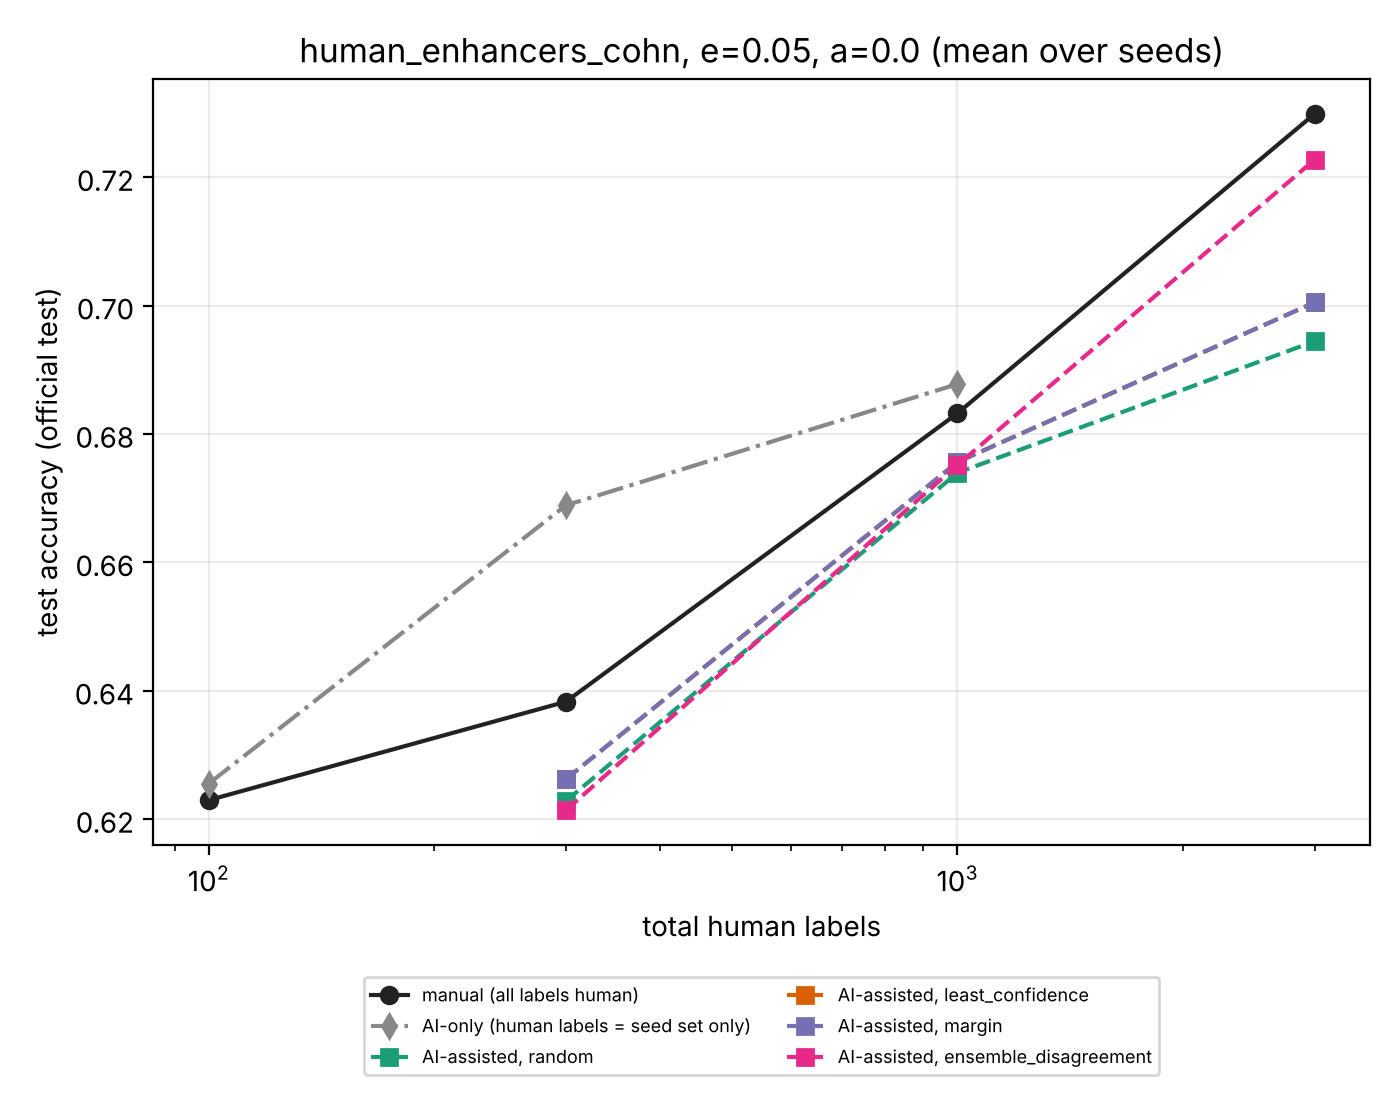
\includegraphics[width=0.78\linewidth]{figures/fig1_accuracy_vs_labels.png}
\caption{Enhancers, main cell ($e=0.05$, $a=0$): mean test accuracy over five seeds against total human labels. Least-confidence coincides with margin (identical selections for two classes) and is hidden underneath it.}\label{fig:acc}
\end{figure}
\begin{table}[t]
\centering\small
\begin{tabular}{lcccc}
\toprule
 & \multicolumn{4}{c}{Total human labels} \\
\cmidrule(lr){2-5}
 & 100 & 300 & 1000 & 3000 \\
\midrule
Manual (all labels human) & 62.3 $\pm$ 4.0 & 63.8 $\pm$ 4.3 & 68.3 $\pm$ 3.7 & 73.0 $\pm$ 0.7 \\
AI-only (human labels = seed set) & 62.6 $\pm$ 3.6 & 66.9 $\pm$ 1.8 & 68.8 $\pm$ 3.5 & -- \\
AI-assisted, random & -- & 62.3 $\pm$ 4.1 & 67.4 $\pm$ 2.3 & 69.5 $\pm$ 2.5 \\
AI-assisted, least-confidence & -- & 62.6 $\pm$ 3.6 & 67.6 $\pm$ 2.5 & 70.0 $\pm$ 3.2 \\
AI-assisted, margin & -- & 62.6 $\pm$ 3.6 & 67.6 $\pm$ 2.5 & 70.0 $\pm$ 3.2 \\
AI-assisted, ensemble disagreement & -- & 62.1 $\pm$ 4.0 & 67.5 $\pm$ 2.4 & 72.3 $\pm$ 1.1 \\
\bottomrule
\end{tabular}

\caption{Test accuracy (\%), mean $\pm$ standard deviation over five seeds, main cell. Least-confidence and margin select identical items and give identical results.}\label{tab:acc}
\end{table}
Table~\ref{tab:acc} and Figure~\ref{fig:acc} give accuracies and Table~\ref{tab:comp} the paired comparisons. Of \nComp{} comparisons, \nFullBeats{} is a clear gain, \nFullWorse{} are clearly worse and \nFullNoClear{} show no clear difference; the low-overlap subset gives the same counts. The single clear gain over random review is ensemble disagreement at the largest budget: \EnsVsRandMean\pp{} (interval \EnsVsRandLo{} to \EnsVsRandHi\pp), positive in \EnsSeedPos{} of 5 seeds (per-seed gains \EnsSeedMin{} to \EnsSeedMax\pp). Least-confidence and margin gain only \LcVsRandMean\pp{} there (interval \LcVsRandLo{} to \LcVsRandHi\pp), with per-seed gains from \LcSeedMin{} to \LcSeedMax\pp. At the two smaller budgets no policy differs clearly from random. Nine policy-versus-random tests were run without correction for multiple comparisons, and the interval treats five seeds as a sample, so one positive result among nine should be read with caution.

\begin{table}[t]
\centering\footnotesize
\begin{tabular}{lccl}
\toprule
Comparison (accuracy, pp) & Mean & 95\% CI & Verdict \\
\midrule
\multicolumn{4}{l}{\emph{Budget pair 100$\to$300}} \\
least-conf. vs. random & +0.34 & [-0.47, +1.11] & no clear difference \\
margin vs. random & +0.34 & [-0.47, +1.07] & no clear difference \\
ens. disagr. vs. random & -0.14 & [-0.76, +0.50] & no clear difference \\
random vs. manual(300) & -1.55 & [-7.55, +3.65] & no clear difference \\
least-conf. vs. manual(300) & -1.21 & [-6.61, +3.76] & no clear difference \\
margin vs. manual(300) & -1.21 & [-6.38, +3.29] & no clear difference \\
ens. disagr. vs. manual(300) & -1.69 & [-7.76, +3.54] & no clear difference \\
AI-only(100) vs. manual(100) & +0.26 & [-3.95, +4.51] & no clear difference \\
\multicolumn{4}{l}{\emph{Budget pair 300$\to$1000}} \\
least-conf. vs. random & +0.17 & [-0.47, +0.79] & no clear difference \\
margin vs. random & +0.17 & [-0.49, +0.79] & no clear difference \\
ens. disagr. vs. random & +0.12 & [-1.03, +1.29] & no clear difference \\
random vs. manual(1000) & -0.93 & [-5.24, +3.03] & no clear difference \\
least-conf. vs. manual(1000) & -0.76 & [-4.98, +3.37] & no clear difference \\
margin vs. manual(1000) & -0.76 & [-4.96, +3.68] & no clear difference \\
ens. disagr. vs. manual(1000) & -0.81 & [-5.32, +3.80] & no clear difference \\
AI-only(300) vs. manual(300) & +3.06 & [-0.82, +7.43] & no clear difference \\
\multicolumn{4}{l}{\emph{Budget pair 1000$\to$3000}} \\
least-conf. vs. random & +0.60 & [-0.43, +1.53] & no clear difference \\
margin vs. random & +0.60 & [-0.37, +1.58] & no clear difference \\
ens. disagr. vs. random & +2.83 & [+1.32, +4.47] & beats \\
random vs. manual(3000) & -3.54 & [-5.49, -1.61] & worse \\
least-conf. vs. manual(3000) & -2.94 & [-5.44, -0.69] & worse \\
margin vs. manual(3000) & -2.94 & [-5.32, -0.48] & worse \\
ens. disagr. vs. manual(3000) & -0.71 & [-1.49, +0.07] & no clear difference \\
AI-only(1000) vs. manual(1000) & +0.45 & [-2.32, +2.71] & no clear difference \\
\bottomrule
\end{tabular}

\caption{Paired comparisons in the main cell on the full test set. Differences in percentage points (positive favours the first arm); 95\% paired bootstrap over seeds and test items; verdict by the frozen rule (gain of at least 1.0\pp{} with lower bound above zero).}\label{tab:comp}
\end{table}

A mechanism check supports the idea that routing finds items the AI gets wrong. The proposer is correct on only \RevPropLc\% of the items chosen by least-confidence and \RevPropEns\% of those chosen by ensemble disagreement, against \RevPropRand\% for randomly chosen items (budget pair 1000$\to$3000), while reviewed labels are about \RevLabLc\% correct, reflecting the 5\% annotator error. Reviewing therefore corrects many errors, but the gain in test accuracy is small because most training items remain pseudo-labelled.

\subsection{RQ2: AI-assisted against manual labelling}
At equal human labels, no AI-assisted arm beats manual labelling (Table~\ref{tab:comp}). At 3{,}000 labels, random, least-confidence and margin routing are clearly worse than Manual(3000) (\RandVsManMean{} and \LcVsManMean\pp{}, intervals \RandVsManLo{} to \RandVsManHi{} and \LcVsManLo{} to \LcVsManHi\pp), while ensemble disagreement is close and not clearly different (\EnsVsManMean\pp, interval \EnsVsManLo{} to \EnsVsManHi\pp). At 300 and 1000 labels the intervals are wide (about $\pm$5\pp) and no difference is clear. AI-only labelling is not clearly better or worse than manual labelling with the same seed set: at $s=300$ it is higher by \OnlyVsManMean\pp{} with an interval of \OnlyVsManLo{} to \OnlyVsManHi\pp. The proposer is a weak labeller (\ProposerAccOneH\%, \ProposerAccThreeH\% and \ProposerAccOneK\% test accuracy for $s=100,300,1000$; Table~\ref{tab:prop}), so roughly 30\% of the pseudo-labels that fill most of the training set are wrong. That is the likely reason why AI-assisted arms trail manual labelling, but we did not test it, since the planned arm without pseudo-labels was not run. Manual($3000$) reaches \ManThreeK\%, close to the \DnaEnh\% of the full-label baseline, which suggests diminishing returns from more labels on this dataset.

\begin{table}[t]
\centering\small
\begin{tabular}{rcc}
\toprule
Seed labels $s$ & Proposer test accuracy (\%) & Pseudo-label accuracy (\%) \\
\midrule
100 & 63.6 & 64.3 \\
300 & 68.1 & 68.5 \\
1000 & 70.5 & 70.6 \\
\bottomrule
\end{tabular}

\caption{Quality of the proposer and of its pseudo-labels in the main cell (mean over seeds).}\label{tab:prop}
\end{table}

\paragraph{Sensitivity to annotator error and reliance.} Table~\ref{tab:sens} gives the gains of two policies over random review for the budget pair 1000$\to$3000 (seeds 0--2, point estimates only). Ensemble disagreement stays ahead of random in \SensEnsAllPos{} cells (\SensEnsMin{} to \SensEnsMax\pp). The advantage is smaller at the higher error rate and when the annotator trusts the AI (reliance 0.3), as expected, since reviewed labels then add less correction. Least-confidence ranges from \SensLcMin{} to \SensLcMax\pp{} and loses its advantage at $e=0.10$.
\begin{table}[t]
\centering\small
\begin{tabular}{ccccc}
\toprule
Error $e$ & Reliance $a$ & Random acc (\%) & Least-conf. gain (pp) & Ens. disagr. gain (pp) \\
\midrule
0.00 & 0.0 & 69.1 & +1.31 & +3.08 \\
0.00 & 0.3 & 69.0 & +0.82 & +1.18 \\
0.05 & 0.0 & 70.2 & +1.15 & +2.59 \\
0.05 & 0.3 & 70.2 & +0.87 & +1.63 \\
0.10 & 0.0 & 69.6 & -0.02 & +1.47 \\
0.10 & 0.3 & 69.5 & -0.27 & +0.55 \\
\bottomrule
\end{tabular}

\caption{Gain over random review, budget pair 1000$\to$3000, seeds 0--2 (point estimates, no intervals).}\label{tab:sens}
\end{table}

\subsection{RQ3: calibration}
\begin{table}[t]
\centering\small
\begin{tabular}{lcccc}
\toprule
 & \multicolumn{4}{c}{Total human labels} \\
\cmidrule(lr){2-5}
 & 100 & 300 & 1000 & 3000 \\
\midrule
Manual & 0.340 & 0.314 & 0.176 & 0.095 \\
AI-only & 0.336 & 0.287 & 0.265 & -- \\
AI-assisted, random & -- & 0.337 & 0.271 & 0.231 \\
AI-assisted, least-confidence & -- & 0.336 & 0.282 & 0.248 \\
AI-assisted, ensemble disagreement & -- & 0.328 & 0.264 & 0.210 \\
\bottomrule
\end{tabular}

\caption{Expected calibration error (15 bins, lower is better), main cell, mean over seeds.}\label{tab:ece}
\end{table}
Models trained with pseudo-labels are markedly worse calibrated (Table~\ref{tab:ece}). At 3{,}000 human labels, ECE is \EceManThree{} for manual labelling and \EceRandThree{}, \EceLcThree{} and \EceEnsThree{} for AI-assisted labelling with random, least-confidence and ensemble routing. AI-only at 1{,}000 labels has \EceAiOnlyOne{} against \EceManOne{} for manual labelling. Ensemble routing has the lowest ECE among the AI-assisted arms. Calibration is measured on the official test set, and we did not test why pseudo-labelled training harms it.

\section{Discussion and limitations}
\textbf{What the evidence supports.} On the enhancer data, uncertainty routing by ensemble disagreement gave a reliable gain over random review at the largest budget and a smaller gain across the sensitivity grid; AI assistance did not beat spending the same human labels on random items, and it reduced calibration. These are results of a simulation, with the limits below.

\textbf{Limits.} (1) The annotator is simulated: errors are random flips independent of difficulty, whereas real reviewers err more on hard items, which are exactly the items routing selects. Reliance is a single probability. (2) One dataset (enhancers), one model family and five seeds; seed variance is large at small budgets. (3) One clear gain among \nComp{} comparisons, with no multiplicity correction. (4) Least-confidence and margin are one policy for two classes. (5) The pseudo-label subsample size (5{,}000), learning rate, epochs and CNN settings are our choices, and the interaction between pseudo-label volume and review is untested. (6) The benchmark's promoter split contains heavy overlap that we could characterise but not trace to its construction; we did not check the model's licence or the model authors' default hyperparameters. (7) Near-duplicate detection used exact 16-mer sharing only, so more distant similarity is not excluded for either dataset.

\section{Reproducibility and AI assistance}
The protocol (\texttt{configs/frozen\_protocol.yaml}, commit \texttt{92e1e49}), code, run records and test-set predictions for all \nRecords{} main-grid runs, the evidence ledger and the decision log are in the accompanying repository. Every number in this paper is generated from the saved result files by \texttt{paper/make\_tables.py}, except the leakage-audit counts in Tables~\ref{tab:leak} and~\ref{tab:strat}, which were transcribed from the student's terminal output of the audit scripts. The research plan, code and this manuscript were prepared with an AI assistant (Claude, Anthropic); the student ran all code on a lab server, supplied all outputs, and is responsible for the content. The assistant's suggestions were logged with their outcomes in the repository's AI-use log. All references were checked against publisher or proceedings pages.

\bibliographystyle{plainnat}
\bibliography{references}
\end{document}
